\openingarticle
\def\ppages{\pagerange{NZAA:firstpage}{NZAA:lastpage}}
\def\shorttitle{Conference Review: New Zealand Archaeological Association}
\def\maintitle{Proceedings from the 2015 New Zealand Archaeological Association Conference}
\def\affiliation{University of Otago}
\def\shortauthor{Jennifer Lane, Helen Heath}
\def\authormail{}%??????
%--------------------------------------------------------------
\mychapter{\maintitle}
\begin{center}
	{\Large\scshape Jennifer Lane\footnote{\href{https://otago.academia.edu/JenniferLane}{Jennifer Lane} is an MA student at the University of Otago in New Zealand. She graduated with a First Class Honours BA in Anthropology (Archaeology), and received a Diploma for Graduates endorsed in Classics. Her research focused on the available methods for investigating non-denominational cemeteries using a pilot study from Dunedin's Historic Northern Cemetery. Jennifer’s current archaeological interests include the monitoring and protection of New Zealand cemeteries and burial grounds, the social transformations surrounding the First World War, and the impact of the 1918 influenza epidemic on New Zealand society.}} \\\href{mailto:lanje121@student.otago.ac.nz}{lanje121@student.otago.ac.nz}\\[1em]
\affiliation\\[1em]
	{\Large\scshape Helen Heath\footnote{Helen Heath is a Masters student at the University of Otago, New Zealand. Helen graduated with a First Class BA Honours in Anthropology, her research included chemical ceramic analysis on assemblages from the Philippines and Thailand. While her current work focuses on Iron Age ceramics from Northeast Thailand, Helen’s interests also include pre-contact New Zealand archaeology and the monitoring and protection of early Maori sites.}}\\ \href{mailto:heahe206@student.otago.ac.nz}{heahe206@student.otago.ac.nz}
\end{center}
\vspace{3em}
\midarticle
%--------------------------------------------------------------
\label{NZAA:firstpage}

\lettrine[nindent=0em,lines=3]{F}{rom} 17--20 June 2015, the \href{http://www.nzarchaeology.org/}{New Zealand Archaeological Association} (NZAA) annual conference took place in Waitangi, Bay of Islands, Aotearoa/New Zealand (Fig. \ref{fig:NZAA_Fig1}). As a site of national significance as the imagined birthplace of the New Zealand nation, Waitangi was chosen as the location for our 2015 conference to commemorate the 170th anniversary of the end of the Northern Wars, the \nth{175} anniversary of the signing of the Treaty of Waitangi, and the \nth{200} anniversary of the establishment of the first mission station (December 1814). The history of Waitangi (Fig. \ref{fig:NZAA_Fig2}) is central to New Zealand’s bi-cultural nationality as the location where British representatives signed a treaty with Maori in 1840 to recognise indigenous land rights.

	\begin{figure}
		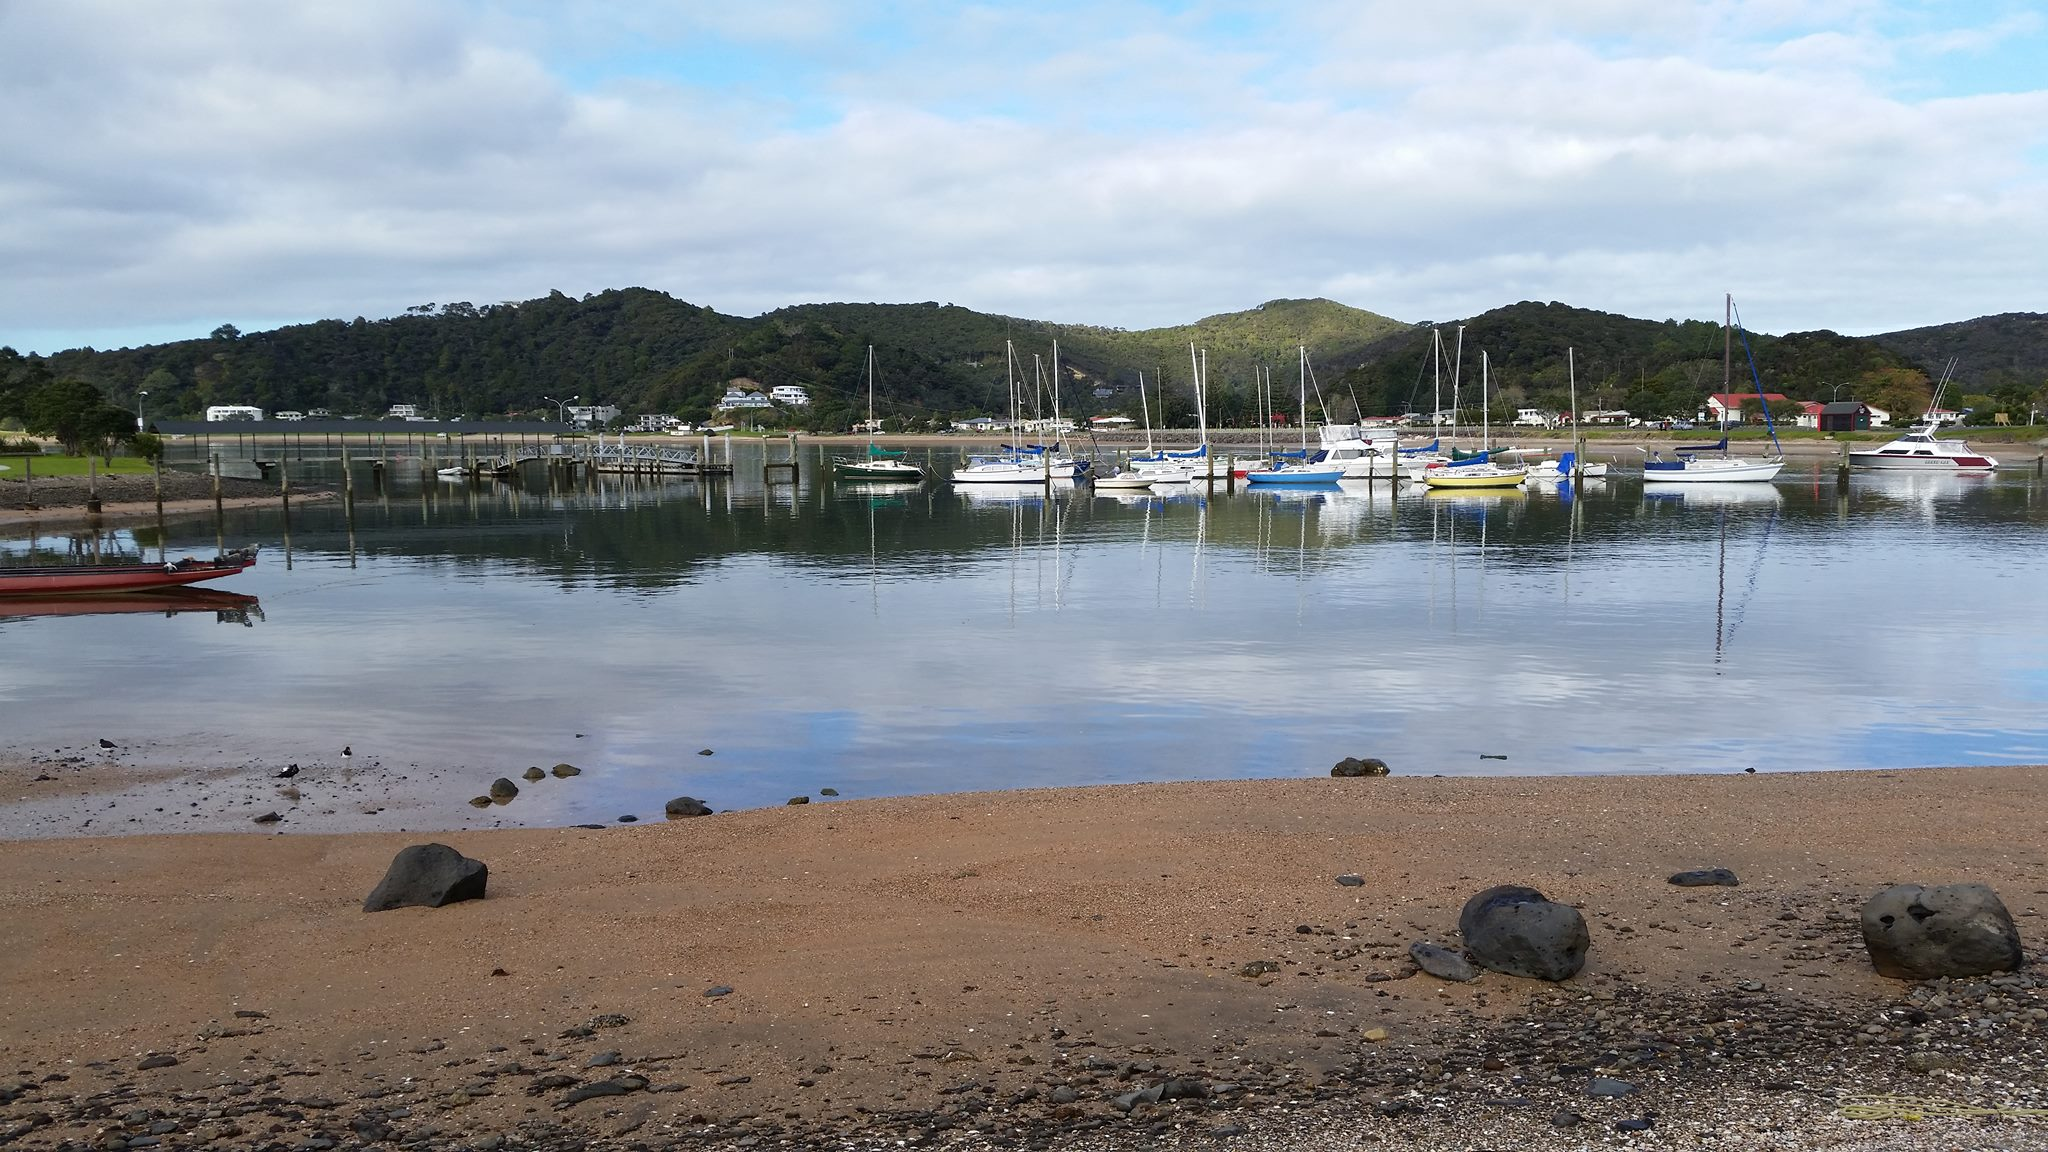
\includegraphics[width=\linewidth]{figures/NZAA_Fig1.jpg}
		\centering
		\caption{View from the Conference Venue. Photo Credit to Naomi Woods.}
		\label{fig:NZAA_Fig1}
	\end{figure}
	\begin{figure}
		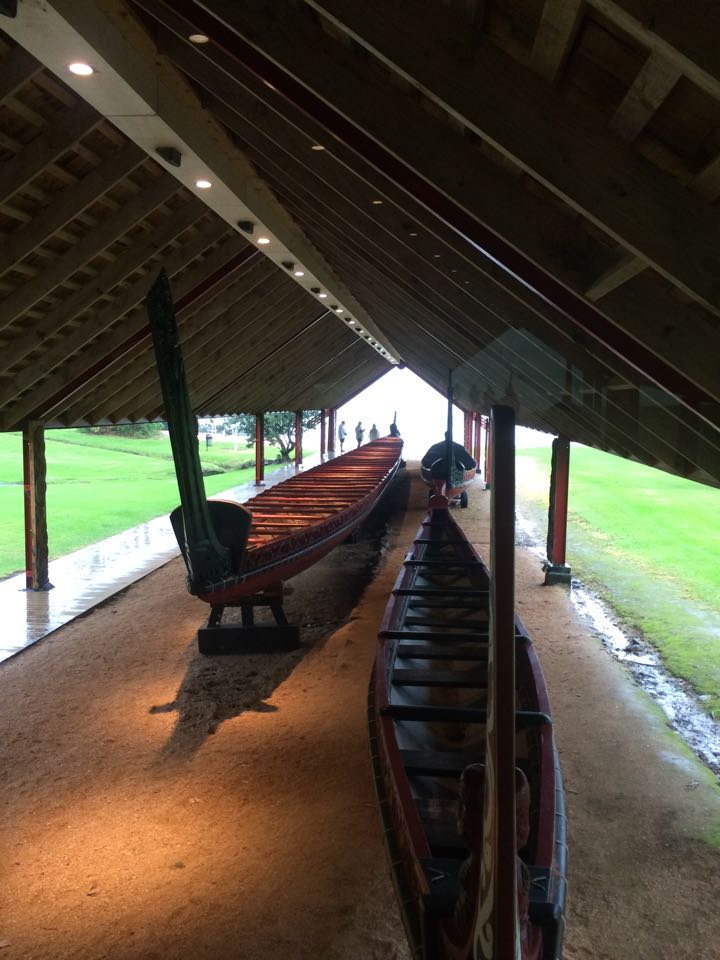
\includegraphics[width=\linewidth]{figures/NZAA_Fig2.jpg}
		\centering
		\caption{Ceremonial war canoe (Ngātokimatawhaorua), at Waitangi. Photo Credit to Jenni Lane.}
		\label{fig:NZAA_Fig2}
	\end{figure}
	
The annual conference field trip visited many local archaeological sites related to the Northern or the First New Zealand War of 1845-46. These trips included visits to the Church Mission Society Mission at Waimate North, and the Ruapekapeka battle site (Figs. \ref{fig:NZAA_Fig3}\&\ref{fig:NZAA_Fig4}). Local guides Kate Martin, Kevin Ashcroft, Stuart Park, and Jonathan Carpenter gave informative talks throughout the trip.

	\begin{figure}
		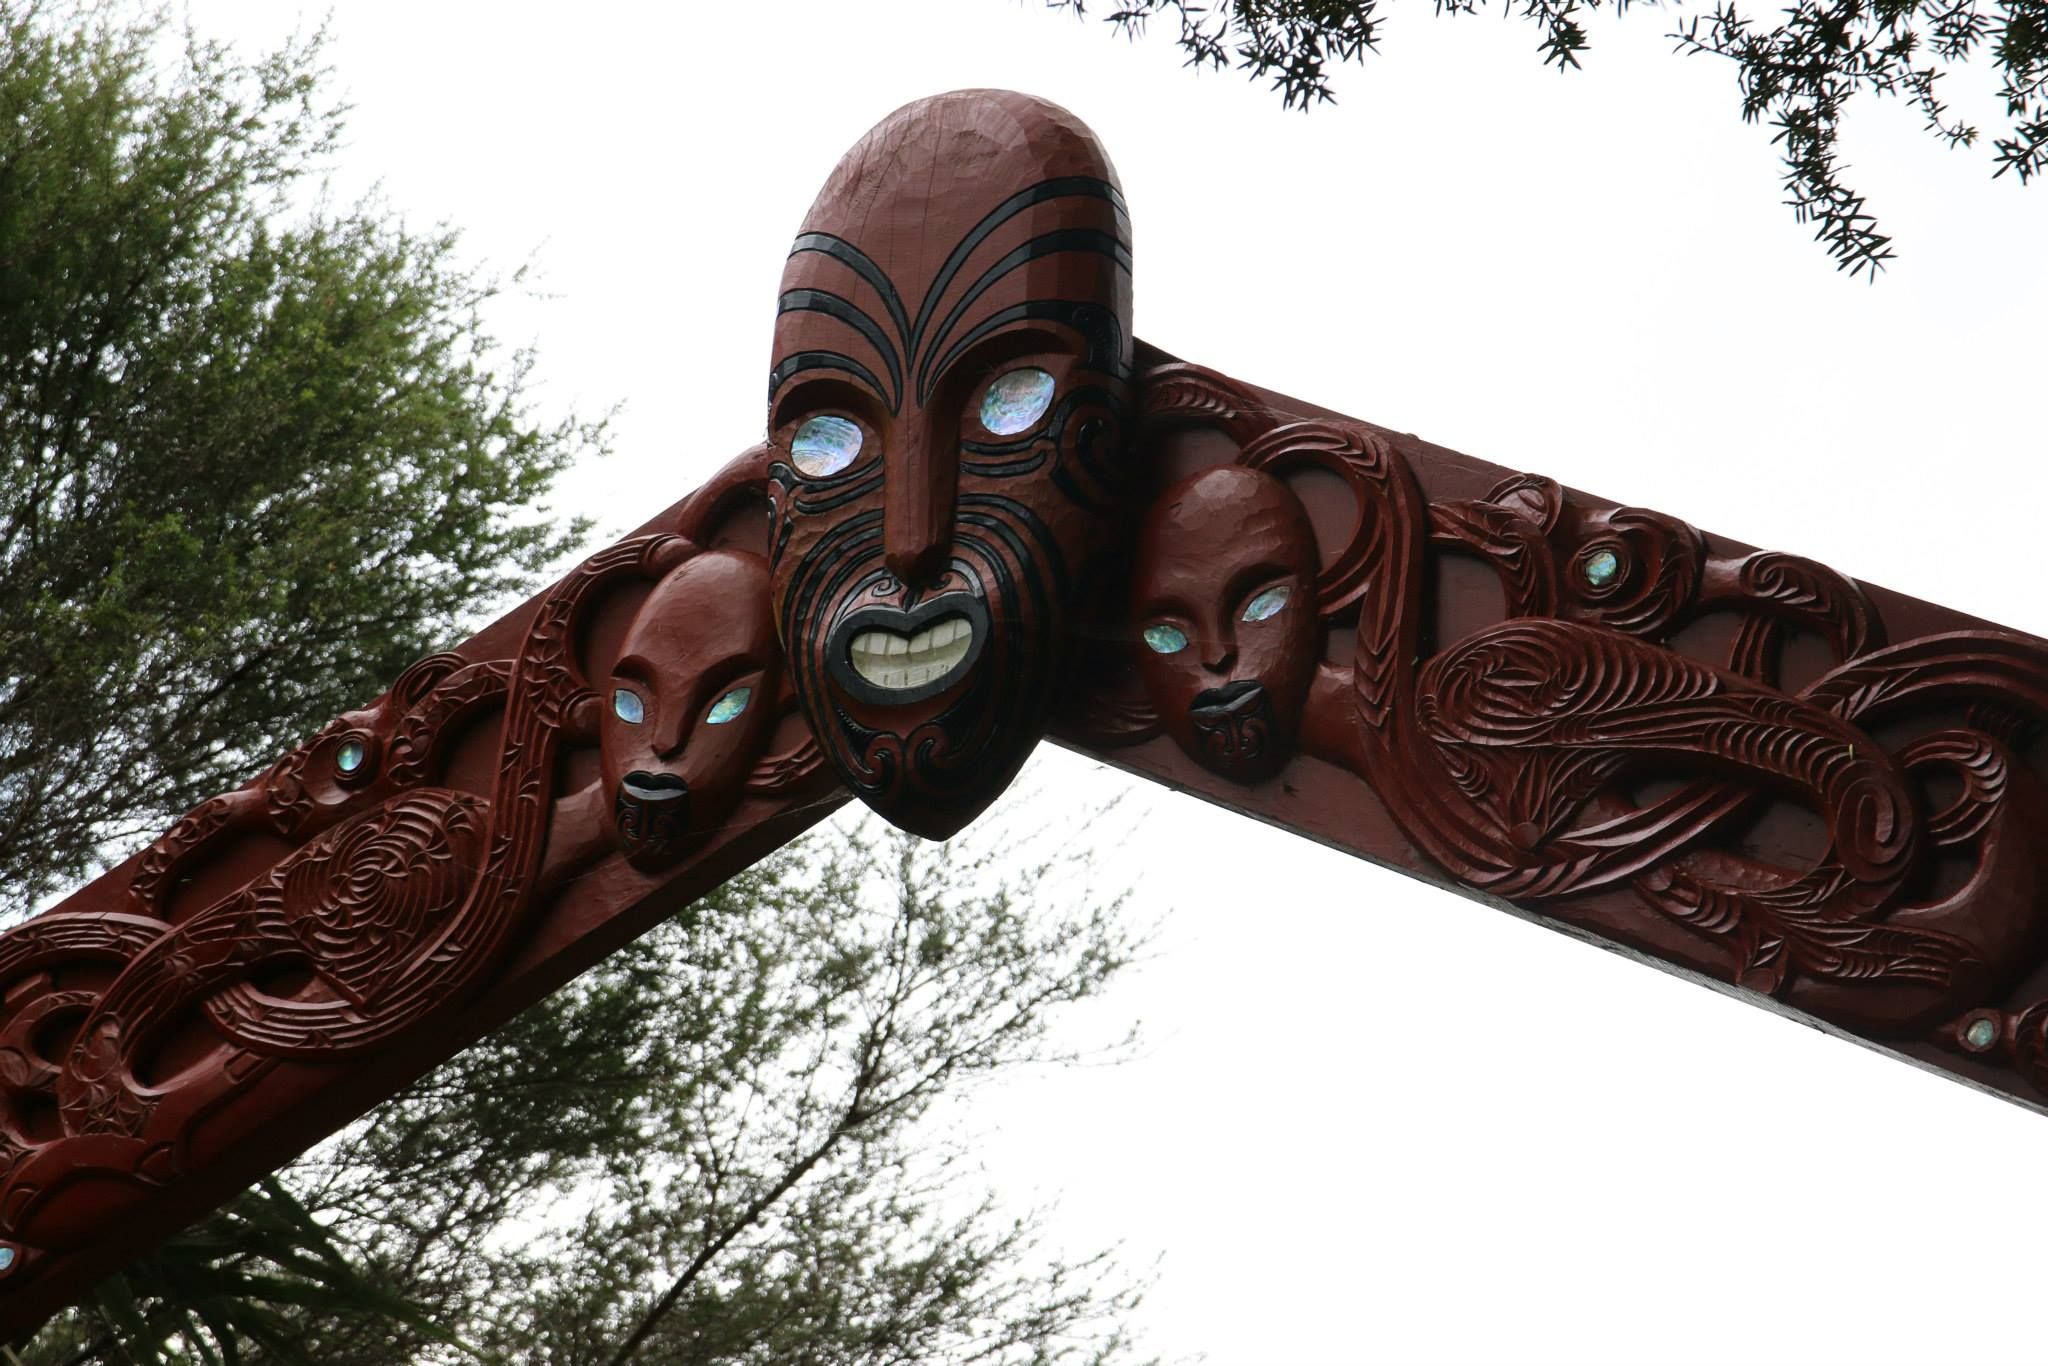
\includegraphics[width=\linewidth]{figures/NZAA_Fig3.jpg}
		\centering
		\caption{Ruapekapeka Pa entrance. Photo Credit to Jean Spinks.}
		\label{fig:NZAA_Fig3}
	\end{figure}
	\begin{figure}
		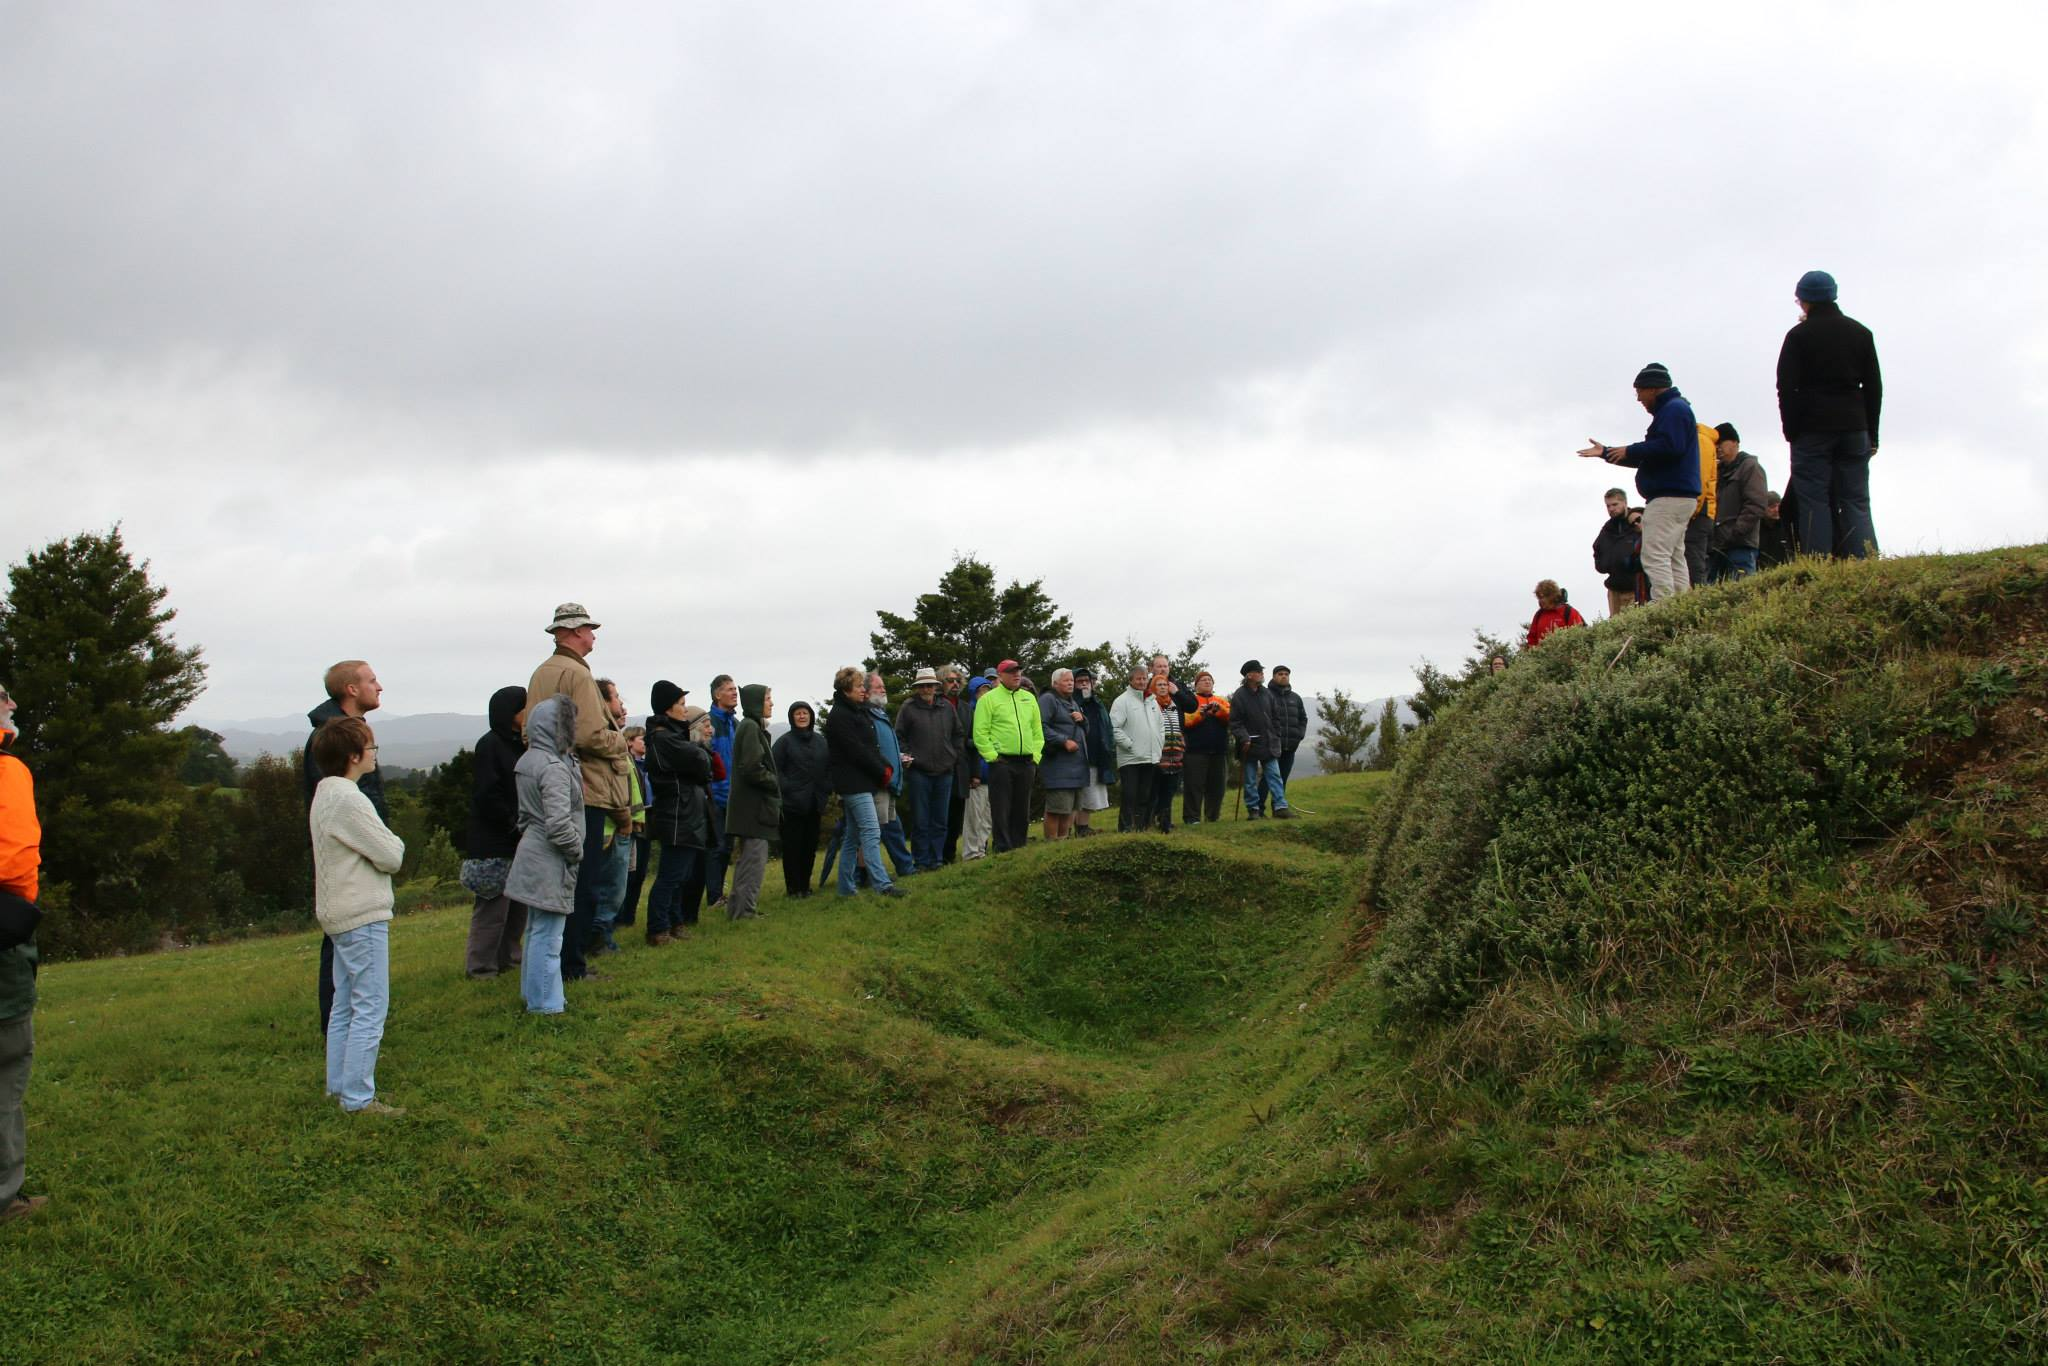
\includegraphics[width=\linewidth]{figures/NZAA_Fig4.jpg}
		\centering
		\caption{Field trip to Ruapekapeka Pa. Photo Credit to Jean Spinks.}
		\label{fig:NZAA_Fig4}
	\end{figure}
	
Conference-goers were also encouraged to visit the Waitangi Treaty Grounds, which was the location of the signing of the Treaty of Waitangi/Te Tiriti o Waitangi. Te Whare Rūnanga (Meeting House) and the Treaty House (Fig. \ref{fig:NZAA_Fig5}) were inhabited by James Busby, as the representative of the British Crown during this era. Ceremonial war canoes are launched from here every year on Waitangi Day (6 February) in commemoration of the signing of the Treaty. Many of the sessions focused on pre-contact (fourteenth to eighteenth centuries \AD) to contact period (post-1769) archaeology in New Zealand to highlight the national and archaeological significance of this region.

	\begin{figure}
		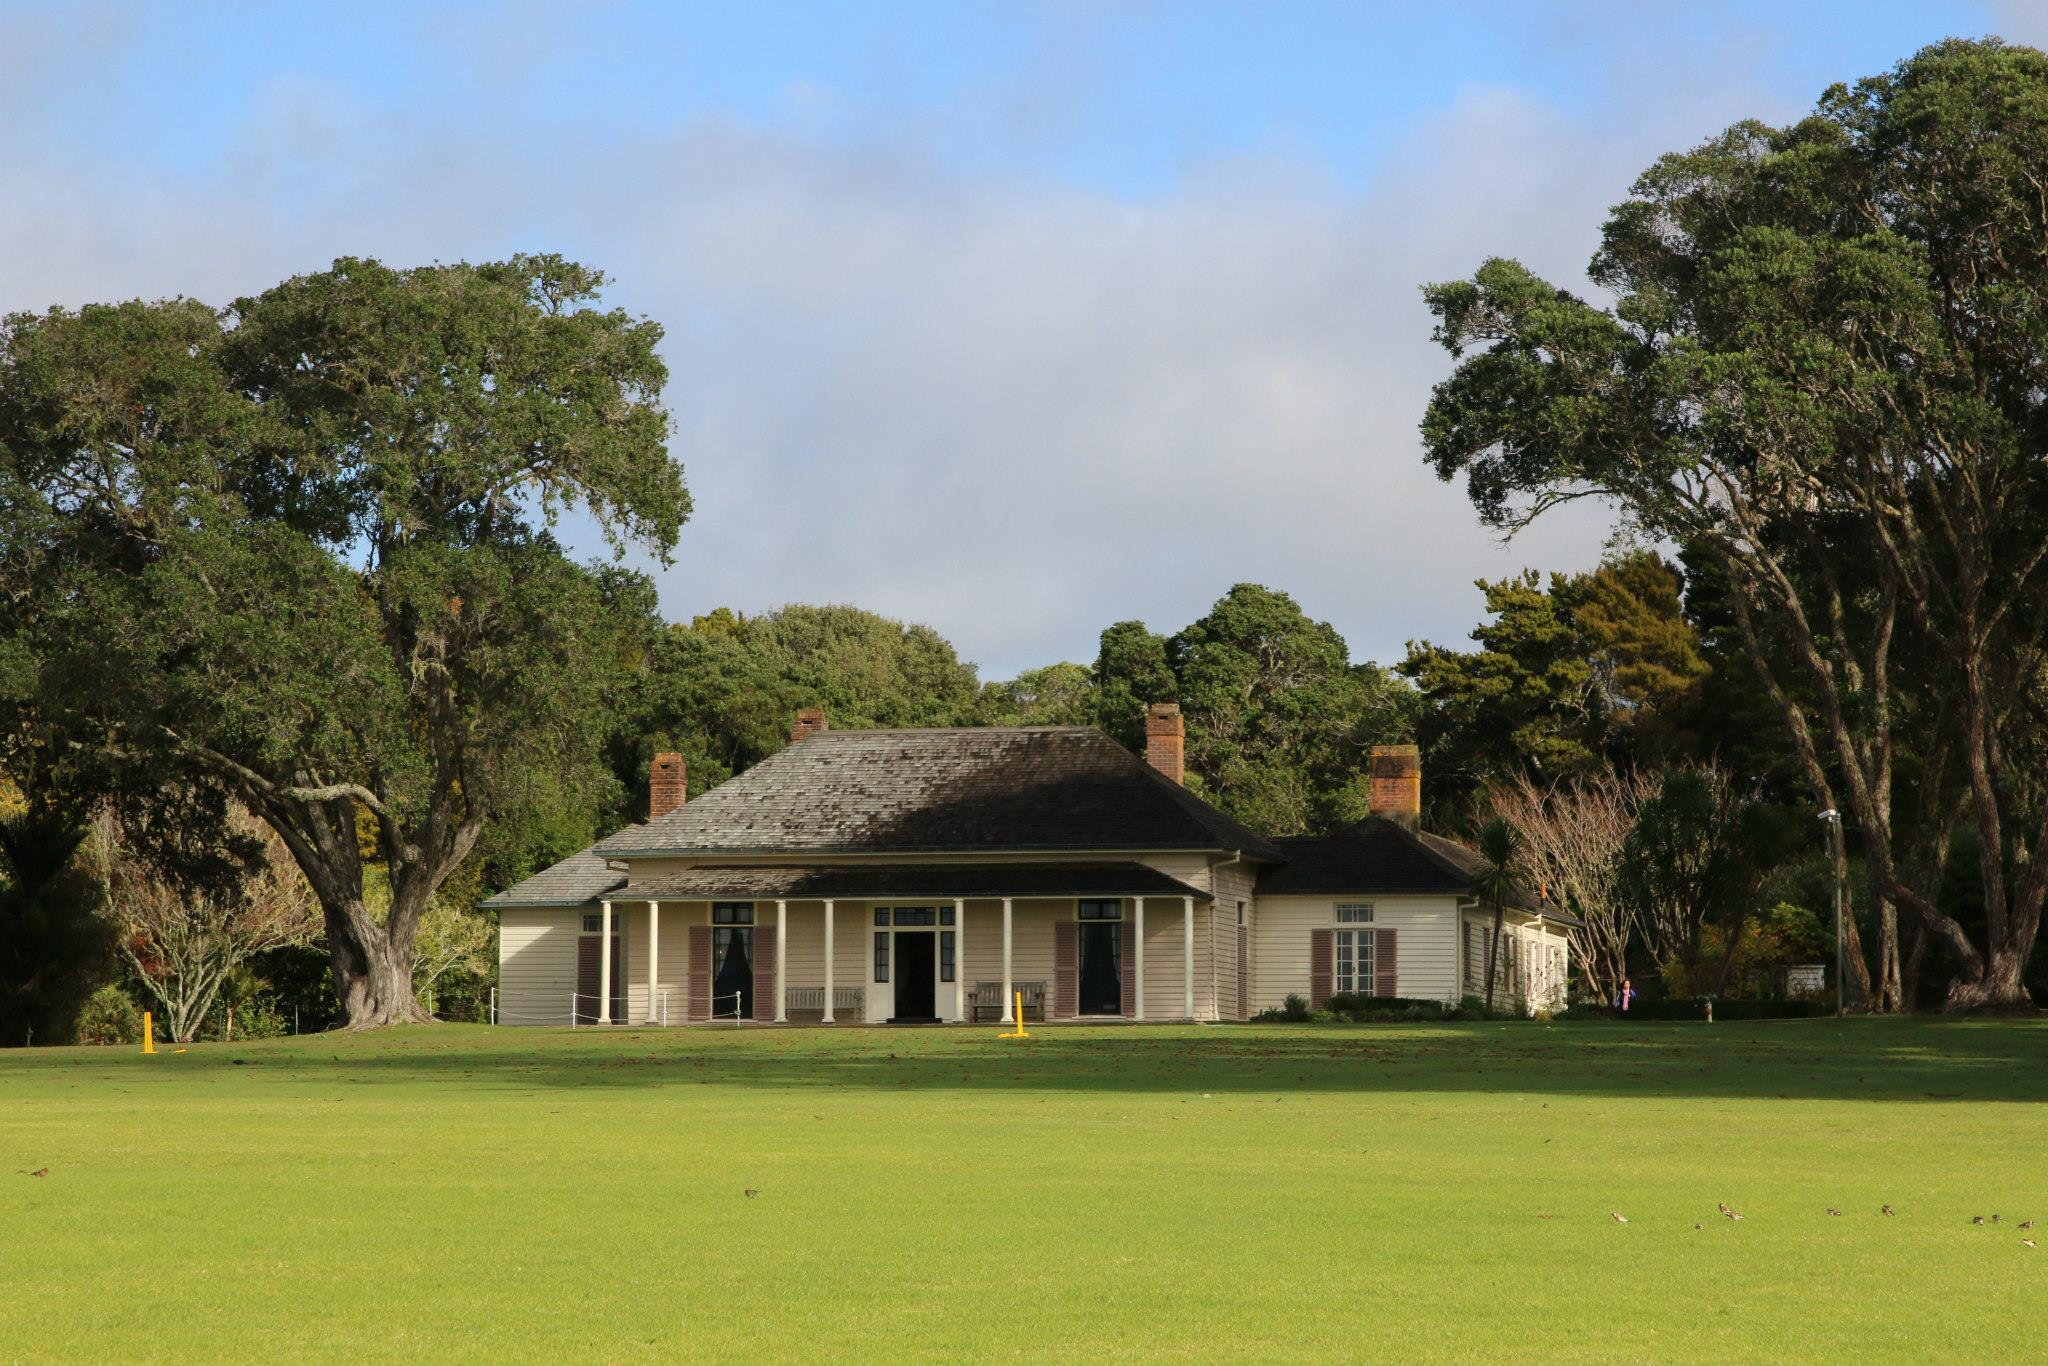
\includegraphics[width=\linewidth]{figures/NZAA_Fig5.jpg}
		\centering
		\caption{The Treaty House, built in 1833. Photo Credit to Jean Spinks.}
		\label{fig:NZAA_Fig5}
	\end{figure}

The conference began on Wednesday with a pōwhiri (traditional Māori greeting) from a representative from Te Tii Marae, followed by the first round of presentations. Presentation topics included: cultural heritage practice, management and further improvements; pre-contact New Zealand archaeology; Bay of Islands archaeology; environmental archaeology, historical archaeology; and material culture studies. 

The student session was introduced in the \nth{60} Anniversary of the New Zealand Archaeological Association conference (2014) for undergraduates and postgraduates to gain experience in presenting papers. These sessions have been reduced from the standard 20 minute presentations to a 10 minute presentation to encourage first time speakers and to promote the research being carried out in our universities.

%\section{Student Session}

The \marginnote{Student Session} student presentation session covered a diverse range of topics, from ceramic analysis in Thailand, to nineteenth century built structures in Ashburton, South Island. Participants in this session included undergraduate and postgraduate archaeology students from \href{http://www.arts.auckland.ac.nz/en/about/subjects-and-courses/anthropology.html}{Auckland University} and the \href{http://www.otago.ac.nz/anthropology/research/archaeology/index.html}{University of Otago}. 

Helen Heath presented her preliminary results on an electron microprobe analysis of ceramics found in Iron Age kilns at Non Ban Jak, Northeast Thailand. With a focus on the kilns excavated, Heath’s research used chemical analysis to describe the nature of pottery production at the site, indicating that potters were producing a variety of forms for local consumption. 

Following the theme of ceramic analysis, Jenny Loader investigated the disappearance of ceramics in the Western Pacific after 1000\BC. In addition to the transformation and subsequent disappearance of Lapita ceramics after reaching Samoa, there is no archaeological evidence for a post-Lapita ceramic industry in this region. However, the presence of ceramics and production technologies continued in Fiji and Vanuatu up until European contact. Loader explored the reasons why this existed, and the social implications for this apparent disappearance. 

Also in Pacific archaeology, Jessie Hurford’s presentation on ‘Houses, Shrines and the Social Landscape of Tetepare, Solomon Islands’ investigated pre-contact to early-contact period sites in New Georgia. Hurford examined the remains of shrine and house architecture on Tetepare, investigating how it reflected socio-political interactions between island polities, particularly surrounding the practice of ritualised head-hunting raids.

The practical uses of LiDAR in the Pacific were outlined by Joe Mills who compared pedestrian survey data and LiDAR data from settlements on Tutuila in American Samoa. He presented a convincing argument for the potential of LiDAR as a means to combat difficulties faced by pedestrian methods, such as dense vegetation and limited visibility, as well as being a tool to re-evaluate the current pedestrian collected site data from Tutuila.  

Luke Tremlett presented the construction phases of the Ashburton Hospital between the \nth{19} and \nth{20} centuries, and the corresponding social transformations and medical innovations that motivated these architectural additions and remodelings. The presentation of Tremlett’s preliminary results regarding the transformations suggest that patient rooms became smaller and specialised over the construction phases with the requirement for ventilation simultaneously decreasing. 

Kurt Bennett used Rangitoto Island as a case study for the re-use of ship parts in holiday cabins around the coast. Many parts were salvaged from clusters of known shipwrecks from the surrounding area, although few locations are identifiable today due to extreme weathering of the remains. Bennett used archaeological and archival data, as well as oral histories to determine which materials survived for possible reuse. Bennett researched the site formation processes at individual vessel sites and re-used material in cabins to help identify any remains of abandoned vessels.

In light of the recent evidence of climatic change from the Intergovernmental Panel on Climate Change (IPCC) (2013), Rebecca Ramsay reported on her assessment of vulnerable coastal sites within the Hauraki Gulf, Auckland. Ramsay applied a coastal vulnerability model to identify three main archaeological site types that require priority in future conservation efforts to protect New Zealand’s coastal heritage.

Matthew Carter (LaTrobe University) presented his research into the motives, strategies and products of Pākehā and Māori entanglement during the shipbuilding period between 1792-1840. Carter’s presentation outlined the historical context, theories and expectations of what his future work will entail. 

%\section{Main Conference Session Topics: \newline Cultural Heritage Practice, Management, and Further Improvements}

Multiple\marginnote{Main Conference Session Topics: Cultural Heritage Practice, Management, and Further Improvements} sessions over the course of the week touched on current cultural heritage issues and management, and suggested ways to improve current practice. New Zealand archaeology has several pieces of legislation that protect our archaeology and cultural heritage. Many parties, such as local and regional councils, Heritage New Zealand/Pouhere Taonga, the Department of Conservation/Te Papa Atawhai, local iwi (tribes), and land developers have conflicting views on how to best acknowledge and manage these heritage sites and excavated cultural material. The balance of these interests is a challenging national issue.

%\subsection{Māoritanga and Archaeology in New Zealand/Aotearoa}

Suggestions\marginnote{Māoritanga and Archaeology in New Zealand/Aotearoa} on how to improve working relationships between local iwi and archaeologists were presented by Huia Pacey and Makere Rika-Heke, which included a discussion on terminology as a continued thread from the 2014 NZAA Conference. The suggested terms ‘pre-pākehā’ or the eurocentric term ‘pre-contact’ to represent the period prior to European contact, were preferred to the term ‘pre-historic’, whose colloquial connotations are insulting to Māori, who are living descendants of the original settlers of New Zealand.

A large part of working in New Zealand archaeology involves continuous consultation with various groups and organisations including local Maori, interested community groups, and legal parties. Ben Teele emphasised the importance of maintaining a dialogue with the community in any situation where we have the ability to converse with the public.

In the last few decades there has been a shift in focus in New Zealand archaeology from pure research to cultural resource management driven by statutory processes. Andrea Farminer suggested updating the current codes of practice for New Zealand archaeologists, and suggested the benefits of introducing a professional body to maintain standards.

%\subsection{New Zealand Transport Authority/Waka Kotahi}

In\marginnote{New Zealand Transport Authority/Waka Kotahi} pre-contact to contact period archaeology, Mary O’Keefe presented preliminary results from her work on the \SI{18}{\kilo\metre} long Kāpiti Expressway for the New Zealand Transport Association/Waka Kotahi (NZTA). O'Keefe presented on the types of sites discovered, and the material analysed by Southern Pacific Archaeological Research (SPAR). O'Keefe's preliminary results provided an understanding of economy in the pre-European environment. Another NZTA project presented by Ann Neill detailed the historical archaeological discoveries resulting from major earthworks projects along the North-western Motorway and Auckland’s CBD, reflecting particularly on the cooperation between companies and governmental bodies invested in these projects. 

%\subsection{Heritage New Zealand/Pouhere Taonga}

An\marginnote{Heritage New Zealand/Pouhere Taonga} illuminating example of cooperation between tangata whenua (local Maori) and the New Zealand Chinese community was presented by Bill Edwards. The SS Ventnor, a mortuary ship carrying 499 Chinese bodies for reburial in their homeland, sank in 1902 southwest of the Hokianga Harbour. This site became protected at the request of the Chinese community through gazettal (where a post-1900 site meets the definition of an archaeological site and is therefore protected as if it were pre-1900 site) under the \textit{Heritage New Zealand Pouhere Taonga Act 2014}. The impetus to protect this shipwreck came from increased visitation by divers and looters fossickers. The bodies of the thirteen crew who died, and some of the deceased Chinese were washed ashore and reburied by the local iwi. Edwards discussed the gazettal process, facilitated through Heritage New Zealand/Pouhere Taonga, in balancing cultural ties to their Chinese homeland while respecting the urupa (burial sites), but also allowing the descendant community access to their ancestors.

Matt Schmidt presented an update of Heritage New Zealand’s ongoing work in Central Otago, outlining the history of sites in the Lower Nevis Valley, possible pre-European moa-hunting camps and Chinese occupation during the gold rush of the 1860s. The rich history of the area is under evaluation, including how to best protect the heritage sites while achieving a balance with the development needs of the district.

Recently, issues have been raised regarding the use of heritage sites as tourist locations or filming in New Zealand. In particular, archaeologists and local councils have collaborated to discuss access permitted to these heritage sites for either public or corporate use. Laura Dawson and Chris Mallows, of the Auckland Council, explained some issues regarding the protocols for filming on heritage sites, and how archaeologists are responsible for ensuring these protocols are adhered to. 

Hayden Cawte, Matt Schmidt, Sheryl Cawte, and Dan Cropper have successfully applied global archaeological authorities to streamline statutory processes in several sites in the Southern region of New Zealand. These authorities allow for greater protection and management of these sites and active collaboration with stakeholders.  

Malcolm Hutchinson reported on the discovery and documentation of 180 previously unknown sites, generating a large amount of textual and graphic data. Many archaeological sites in New Zealand remain unknown and are unrecorded as they are not visible from the surface; therefore, accidental discoveries occur frequently. This led Hutchinson to develop an experimental software package for the storage and access of this data, and long-term preservation of computational archaeological material. 

Similarly, Benjamin Jones, Shannon McColley, and Igor Drecki presented a new digital resource for cartographic material. As many of these documents are subject to copyright and ownership issues, or are resources unknown to archaeologists, Jones, McColley, and Drecki, in collaboration with the Auckland University digitised approximately 16,000 historical governmental maps in Auckland University Library and the National Library of New Zealand/Te Puna Mātauranga o Aotearoa. 

%\section{Pre-Contact New Zealand Archaeology}

The\marginnote{Pre-Contact New Zealand Archaeology} session started with a presentation on the recent excavation of a nationally significant find, Dilys Johns (Auckland University), Rachel Wesley (Te Rūnanga o Ōtākou) and Shar Briden (Department of Conservation/Te Papa Atawhai). A c.\SI{6}{\metre} long tōtara waka (canoe) was excavated from the sand dunes of Papanui Inlet on the Otago Peninsula in October 2014. Local iwi, archaeologists and conservation specialists worked together to recover the pre-contact waka, which is the second oldest in New Zealand. Along with the waka recovery, Johns also reported on the future preservation of the waka and the continual monitoring of the culturally significant and eroding site of Papanui.    
  
Wrapping up his doctoral thesis this year, James Robinson (Winner: best paper) presented his research on the Poor Knights Islands. Using an archaeological landscape approach paired with traditional and historical records and earth sciences, Robinson mapped and assessed the inaccessible and densely vegetated Tawhiti Rahi Island. The information Robinson gathered was used to identify the various uses of the island through time, such as garden outliers, muttonbird resource areas, horticultural settlements, defence and pig farming. This research was used to describe the relationship of the Poor Knights Islands to the mainland and other surrounding island groups.
Inspired by his previous work on the old telegraph system across the Coromandel Ranges, David Wilton explored a different form of information technology this year. Wilton compared visual signalling technologies used by early Māori with other communities, such as the use of fire among the Chinese and the North American Indians. Wilton also received the Public Archaeology Award for his long term work bringing the archaeology of the Thames Goldfields to the general public.

Kevin Jones presented an update on his work on the Northern Mahia Peninsula. Jones discussed various sites and their significance in contributing to understanding the area’s archaeology. In particular, Jones noted the favoured quincunx patterns of taro cultivation, the landing sites from early occupation, and the positioning of outlier settlements in relation to the mission and whaling stations occupied during the 1840s. 

Using data from shore whaling sites, Garry Law reported on his investigation into early settlement sites in New Zealand, through the use of modelling to assess the frequency of site loss. He left the audience to ponder how much we really know about early sites in New Zealand.

%\section{Bay of Islands Archaeology}

The\marginnote{Bay of Islands Archaeology} presentations of fieldwork undertaken in the Pēwhairangi (Bay of Islands) area focused primarily on the initial contact between Pākehā and local iwi. The town of Paihia (Fig. \ref{fig:NZAA_Fig6}), on the southern bank of the Waitangi River, was the location of the \nth{3} Church Missionary Society Mission Station and a pā site. Unfortunately, the exact position of the pā site has been lost; however, recent investigations by Caroline Phillips have evaluated likely site locations. Through the study of historical images, written accounts, and reconstructing the landscape using known landmarks, Phillips has worked on locating the site, thought to be in the middle of the Paihia township. Several accounts mention the presence of defensive structures, due to rumours of attacking southern tribes, while historical images show the presence of a flagpole. According to written accounts, the site was occupied by Māori and missionaries at separate times, and the site itself transformed in use over its occupation period.

	\begin{figure}
		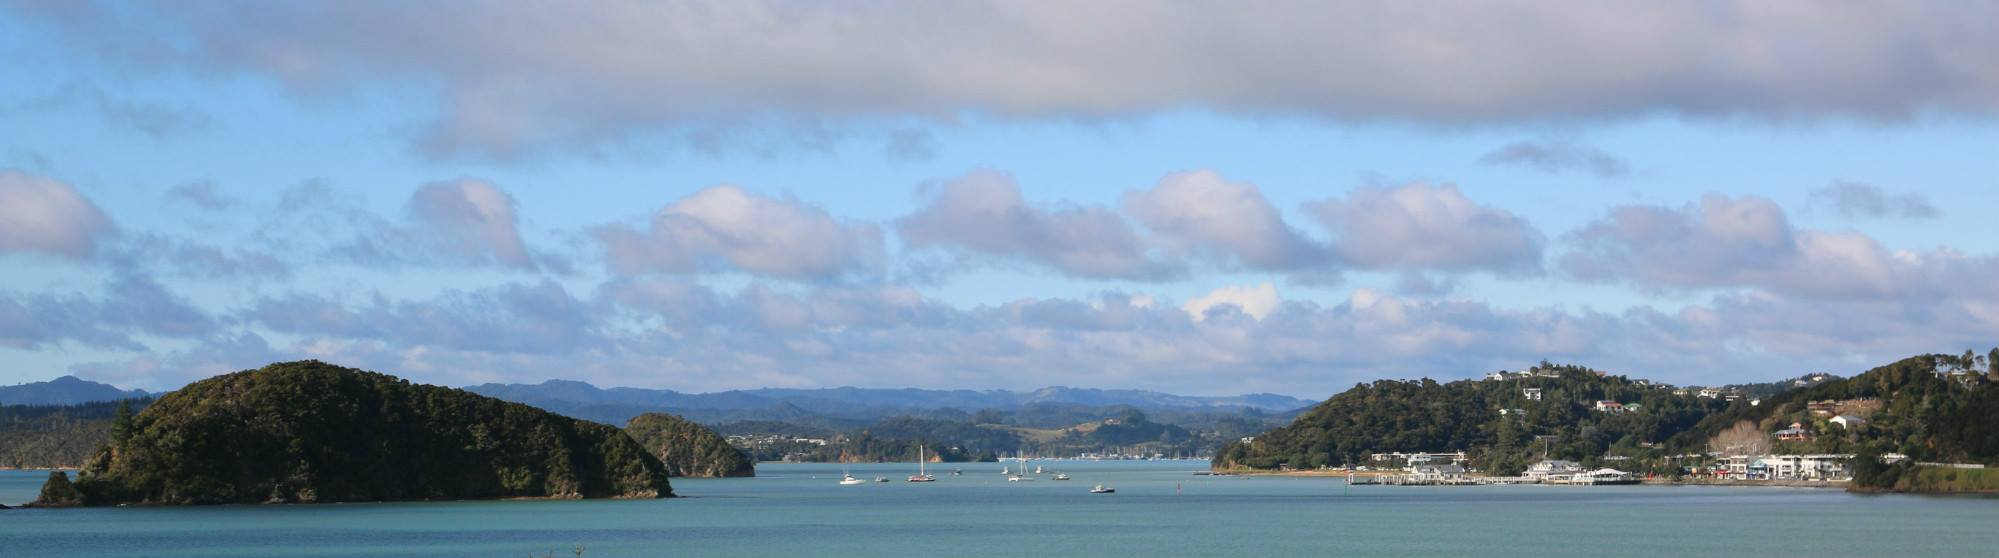
\includegraphics[width=\linewidth]{figures/NZAA_Fig6.jpg}
		\centering
		\caption{View of Paihia. Photo Credit to Jean Spinks.}
		\label{fig:NZAA_Fig6}
	\end{figure}
	
Angela Middleton and Ian Smith both discussed other mission stations located within the area, particularly ones at Hohi and Paihia, which were occupied between 1814 and 1845. Middleton followed the path of missionaries Marsden and Nicholas inland from Paihia towards Waimate, focusing particularly on the relationship between Marsden and the local iwi, Ngāpuhi. Middleton noted the transformations in the political situation of Ngāpuhi through Marsden's diaries and images during the years after contact. 

Smith examined evidence of the political economy present in the Bay of Islands during the early \nth{19} century in relation to the rise and decline of Rangihoua pā. Te Puna village was considered the centre of operations in the Northern area, and even termed the ‘capital’ by a visitor in 1805. Smith’s discussion of agricultural and horticultural trade networks, particularly the settlements with extensive gardens, as opposed to those with coastal resources, indicated that the alliance between the north and south offered a balance of land and sea resources from trade networks, eventually overcoming the limited resources of the eastern tribes.

John Booth’s presentation consisted of a comprehensive overview of the marine ecosystems present in the Bay of Islands, with particular reference to pre-contact coastal sites across the bay. Booth noted that the content of marine resources consumed at pre-contact sites were comparable with Smith’s theories of the wider Hauraki Gulf with particular reference to Mangahawea (\AD 1260-1350), Opunga (\AD 1402-1455), Wairoa (\AD 1390-1455), and Patunui (\AD 1450-1500). The midden analyses of these sites displayed a transformation, from a wide variety of fish and shellfish species plus marine mammals and moa bones, towards a limited consumption of a small range of estuarine shellfish species.

Matthew Campbell presented a case study on fish identification from Parton Road (Papamoa) and Urquharts Bay (Whangarei Harbour). The standard method of identification in New Zealand includes five major mouthparts for a cross-assemblage and cross-site comparison. Campbell extended this method to include cranial and sub-cranial bones, plus vertebrae, for a more successful identification of species across multiple contexts.    
  
Lindsay Alexander investigated the historic 1820s-1880's whale ships, which docked seasonally at north-east ports in New Zealand. The presence of these ships in Northland transformed the society and culture of the towns: where whalers docked had a significant impact on the economic state of the wider communities. The economic structure of towns such as Russell and Mangonui relied heavily on the presence of these ships to thrive, and for the identity of their people. Alexander argued that there were a greater number of ships that docked in the north-east coast of New Zealand than previously known, forcing the towns in the area to transform their identities into cosmopolitan ports. The decline of whale ships arriving in New Zealand ports may have reduced the presence of whalemen in New Zealand, but their unique culture had already made their mark. 

%\section{Environmental Archaeology}

Mark\marginnote{Environmental Archaeology}
 Horrocks presented a macro-botanical approach to compare environmental and agricultural evidence in archaeological excavations in the Pacific. Horrocks argued that pollen, phytolith, and starch grain analyses may be used to identify material discovered in archaeological sites with both wet and dry environments. These three analyses cost the same as standard radiocarbon analysis and are valuable tools for discovering a range of preserved material, due to the diverse number of methods for micro-botanical preservation. The benefit of using these methods in an archaeological context provides useful chronological and environmental information, specifically that of the horticultural actions of early populations. For example, in New Zealand these methods have identified early Māori cultigens and introduced European plants, while across the Pacific, these analyses have been carried out on a range of sources on various islands from New Guinea to Hawai'i.

Rod Wallace’s analysis of material from pre-European horticultural sites in the Waikato (Central North Island) indicated an unusual gardening pattern practice. Wallace identified where land was cleared in the existing Tawa/Mataī bush for a one-off horticultural use, which differs from the northern North Island gardening practice which utilises the same garden multiple times.

For several seasons, the University of Auckland in partnership with the Auckland Museum, have carried out multiple field schools on Ahuahu (Great Mercury Island). Louise Furey, Alex Jorgensen, Rebecca Phillipps, Simon Holdaway, Rod Wallace, and Josh Emmitt are the primary archaeologists associated with this field school. In further research, Isaac McIvor and Thegn Ladefoged have investigated the land use and settlement patterns of the site using a multi-scalar approach of a \SI{300}{\hectare} area. The impacts of the communities on the environment was discovered through categorising the landscape with regards to mobility, storage, competition, and cooperation. The identification of the best locations for horticultural production evaluated the area in \SI{25}{\metre} by \SI{25}{\metre} squares for insolation (sunlight exposure), soil composition, slope, and access to streams. The results of this spatial analysis with the notation of storage pits, residential features and fortified locations indicated that the island was occupied on a continuous basis rather than seasonally.

%\section{Historical Archaeology}

Two\marginnote{Historical Archaeology} key themes were present in the historical archaeology presentations: aspects of New Zealand’s early conflicts, and recent investigations into buildings archaeology. Jonathan Carpenter presented an update of his fieldwork in Ruapekapeka, which included the location of several areas of significance during the Northern or First New Zealand War 1845-46 between the British and Māori allies, and the local iwi. Alexy Simmons investigated the food security of soldiers during campaigns in the Waikato region, particularly the methods used to store, distribute, and ensure a continual supply of food. 

Katherine Watson presented an overview of the work carried out by Underground Overground Archaeology over the last four years in post-earthquake Christchurch. Watson looked into the wider implications and understanding of Christchurch’s history, through the structures and features of the documented domestic houses. Patrick Harsveldt from Opus international Consultants reported on the recording prior to and during demolition of a pre-1900 farmhouse, which gave further insight into the style of building practiced in rural Canterbury during the late 1800s-1900s.

Another aspect of historical archaeology was addressed by Maddy Fowler, who looked into Aboriginal influences on maritime archaeology at mission stations in South Australia. This topic explored a niche that has not been investigated, and she concluded that in these situations it is crucial to work with the local indigenous people for a more comprehensive understanding of the context. Indigenous people living at the Point Pearce Aboriginal Mission/Burgiyana merged indigenous and western maritime practices, which have not been investigated as part of mission archaeology, nor part of maritime archaeology. Fowler has investigated the applicability of western concepts in maritime archaeology to indigenous missions, and its applicability to New Zealand maritime archaeology.

%\section{Material Culture Studies}

Nicholas\marginnote{Material Culture Studies} Sutton (Winner: Best Student Presentation) in collaboration with supervisors Glenn Summerhayes and Anne Ford presented their current work on ceramic production and mobility at Oposisi, Papua New Guinea. Through a stylistic, fabric and chemical analysis, Sutton was able to report preliminary results on a new ceramic sample from Oposisi, in turn investigating the dates for the first settlement and the earliest ceramic horizon, Early Papuan Pottery (EPP).  

Political movements in Christchurch, while well recorded, are not always reflected as vividly in the archaeological record. In light of the discovery of a clay pipe assemblage depicting international political figures and ideal excavated at 152 Armagh Street, Jessie Garland was able to link material culture as a means to reinforce political ideas in \nth{19} century Christchurch. Following in the theme of historical material culture, Naomi Woods led the audience through the gardens depicted on popular Willow pattern tableware. Woods described the influence of the plants and structures in the pattern pertaining to the decision-making process of ornamental garden design in \nth{19} century Whanagnui. 

\SetBlockThreshold{1} 
\blockquote{\textit{The conference ended with a formal dinner and awards for the best papers. The main sponsors were the New Zealand Transport Agency/Waka Kotahi, Far North District Council/Te Kaunihera o Tai Tokerau Ki Te Raki, CFG Heritage, Heritage New Zealand/Pouhere Taonga, Clough \& Associates Ltd., and Heritage Survey Consultants (HSC), whose contributions made this year’s conference possible. 
\\\newline Many thanks to the Copthorne Hotel for hosting, and to Brooke Jamieson for organising the 2015 conference.}}


\label{NZAA:lastpage}
%----------------------------------------------------------------------------------------
\closingarticle